%!TEX program = xelatex
% 完整编译: xelatex -> biber/bibtex -> xelatex -> xelatex
\documentclass[lang=cn,a4paper,newtx]{elegantpaper}

\title{DeepSeek-R1:通过强化学习激励大语言模型的推理能力}
\author{左元翻译}

% 本文档命令
\usepackage{array}
\newcommand{\ccr}[1]{\makecell{{\color{#1}\rule{1cm}{1cm}}}}

\newcommand{\dsri}{DeepSeek-R1}
\newcommand{\dsro}{DeepSeek-R1-Zero}

\begin{document}

\maketitle

\begin{abstract}
  本文介绍了我们的第一代推理模型,\dsro{} 和 DeepSeek-R1。\dsro{} 是通过大规模强化学习(RL)训练的模型,在没有使用监督微调(SFT)这个前置步骤的情况下,展示了卓越的推理能力。通过强化学习,\dsro{} 自然而然的展现出了许多强大而有趣的推理行为。然而,它也面临一些挑战,如可读性差和多语言混合等问题。为了解决这些问题并进一步提高推理性能,我们引入了 DeepSeek-R1,该模型在强化学习之前结合了多阶段训练和冷启动数据。DeepSeek-R1 在推理任务中的表现与 OpenAI-o1-1217 相当。为了支持研究社区,我们开源了 \dsro{}、DeepSeek-R1 以及六个稠密模型(1.5B、7B、8B、14B、32B、70B),这六个稠密模型是使用 \dsri{} 对 Qwen 和 Llama 蒸馏而来。
\end{abstract}

\begin{figure}[h]
\centering
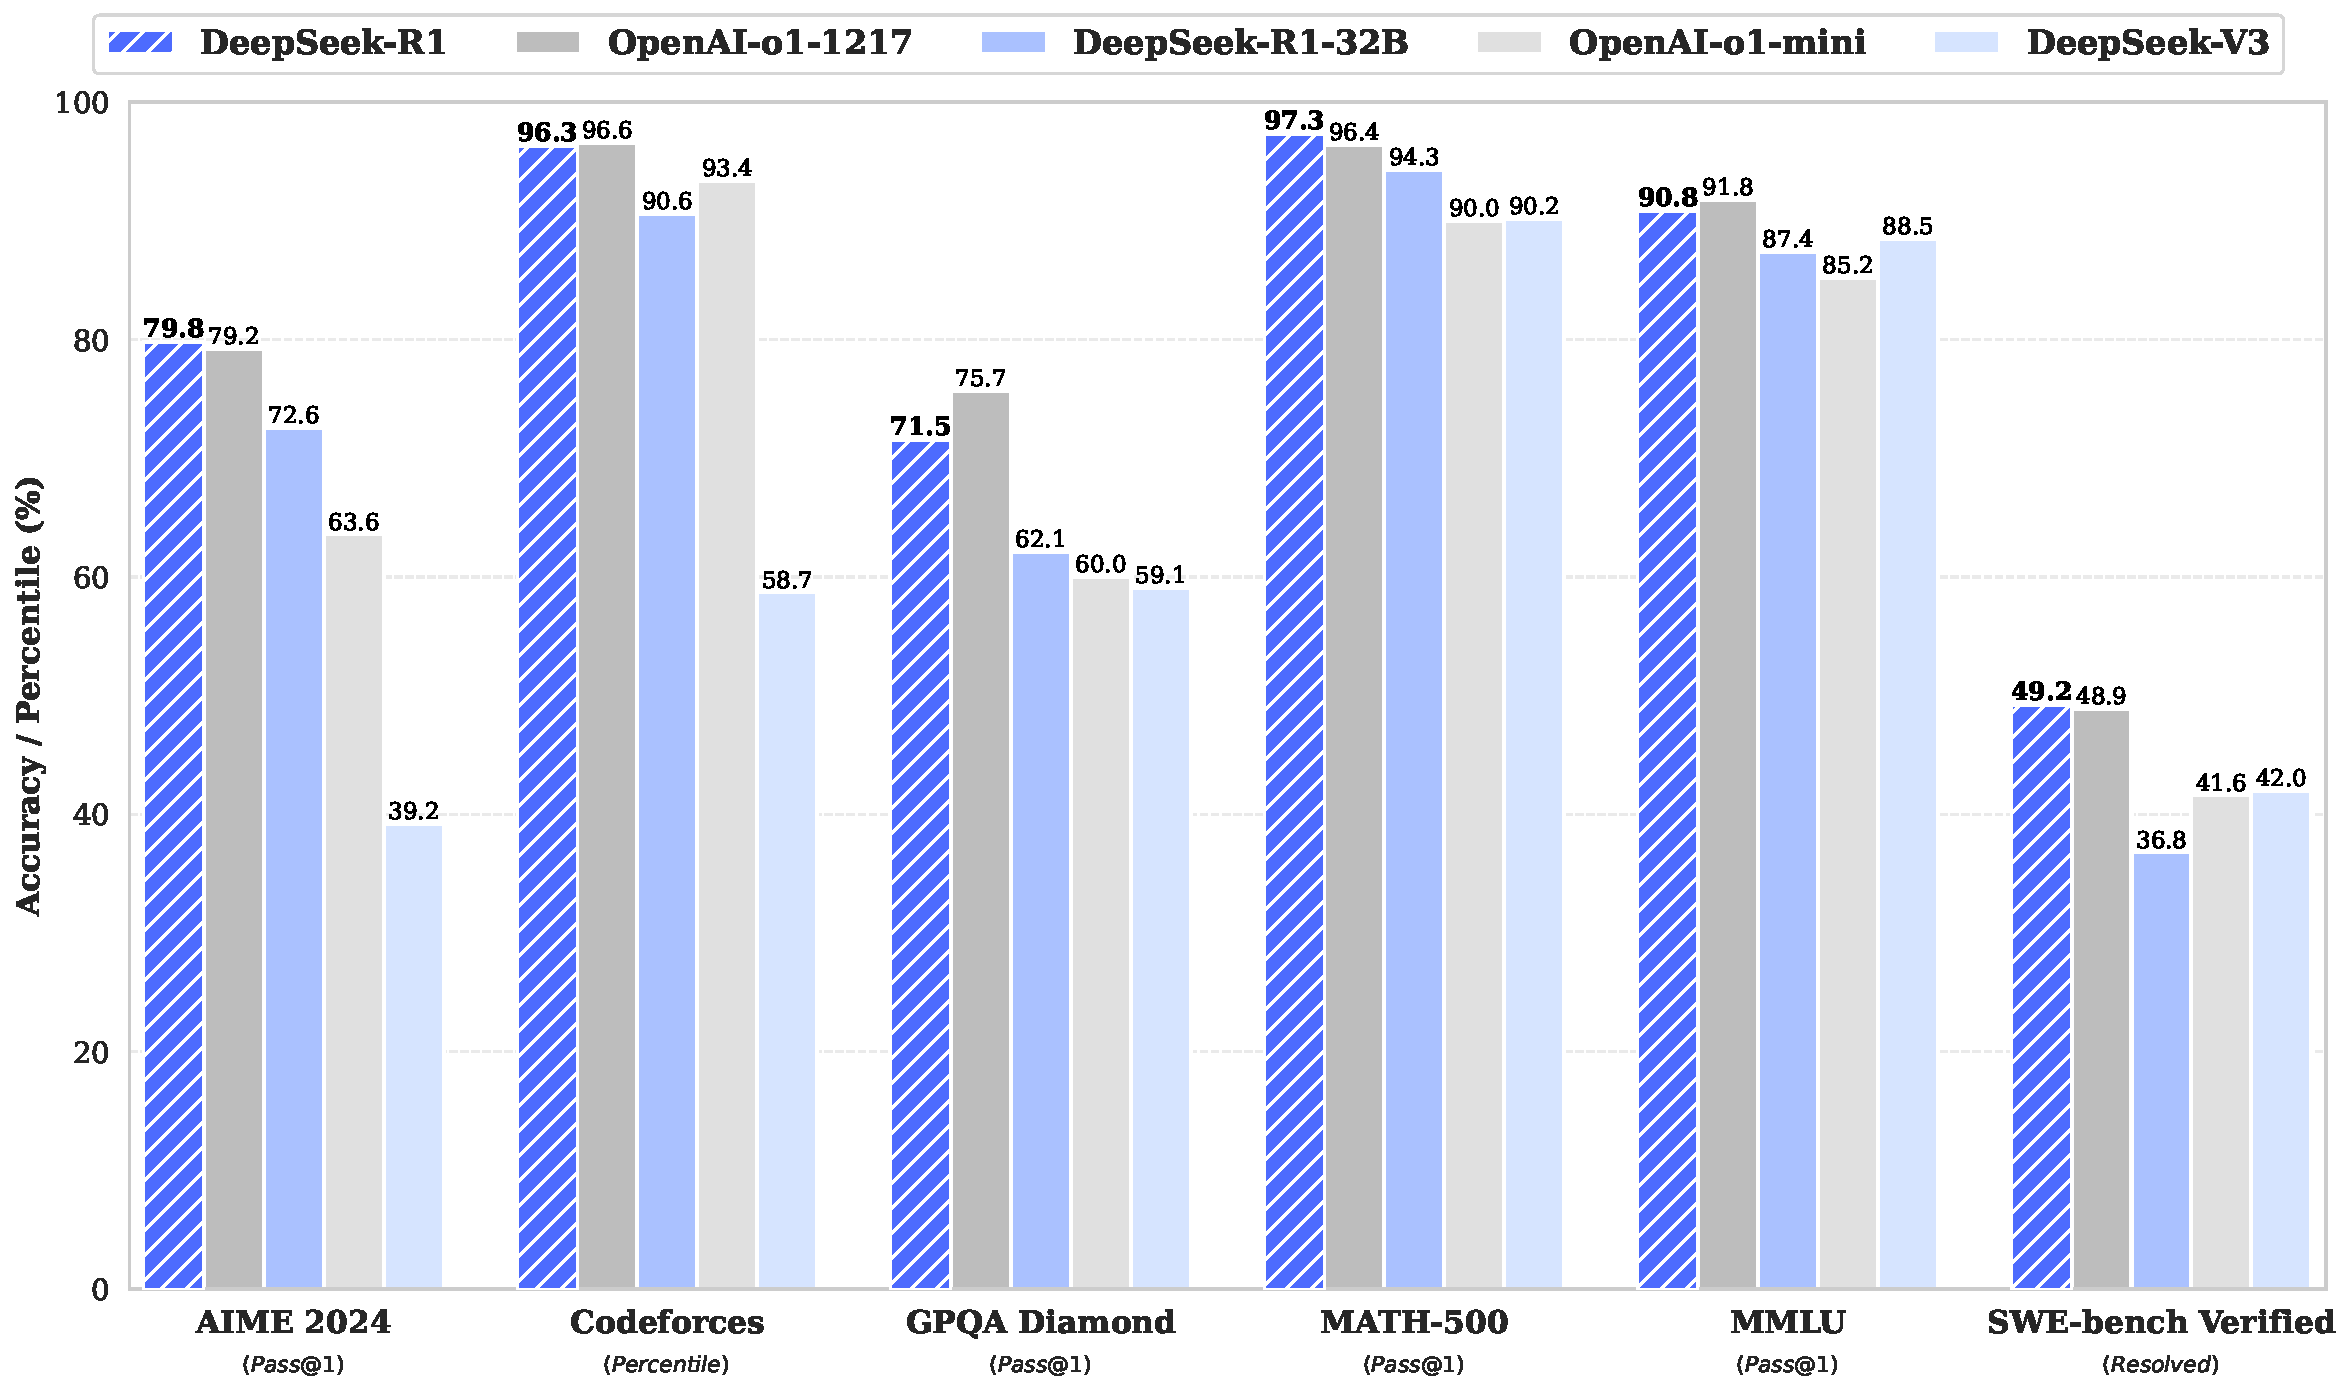
\includegraphics[width=1.0\textwidth]{figures/dsr1_performance.pdf}
\caption{
    \centering
    Benchmark performance of \dsri{}.
}
\label{fig:dsv3_performance}
\end{figure}

\newpage

\tableofcontents

\newpage

\section{简介}

近年来,大语言模型(LLMs)正在经历快速的迭代和进化,并正在逼近通用人工智能(AGI)。

最近,后训练已成为完整训练流程中的一个重要组成部分。研究表明,它可以提高推理任务的准确性,与社会价值观保持对齐,并适应用户偏好,同时相较于预训练所需的计算资源相对较少。在推理能力方面,OpenAI 的 o1 系列模型通过增加思维链推理过程的长度,首次引入了推理时扩展的方法。这种方法在数学、编程和科学推理等多种推理任务中,取得了显著的进步。然而,有效的测试时扩展仍然是社区面临的一个未解问题。之前的一些研究探索了各种方法,包括基于过程的奖励模型、强化学习,以及蒙特卡罗树搜索和束搜索等搜索算法。然而,这些方法都未能实现与 OpenAI 的 o1 系列模型相当的通用推理性能。

在本文中,我们迈出了提升语言模型推理能力的第一步,也就是采用纯粹的强化学习。我们的目标是探索大语言模型在没有任何监督数据的情况下发展推理能力的潜力,重点关注它们通过纯粹的强化学习过程的自我进化。具体而言,我们使用 DeepSeek-V3-Base 作为基础模型,并采用 GRPO 作为强化学习框架,以提高模型在推理方面的性能。在训练过程中,\dsro{} 自然而然的展现出了许多强大而有趣的推理行为。经过数千步的强化学习训练,\dsro{} 在推理基准测试中表现出色。例如,AIME 2024 的 pass@1 分数从 15.6\% 提高到 71.0\%,并且通过多数投票,分数进一步提升至 86.7\%,与 OpenAI-o1-0912 的表现相匹配。

然而,\dsro{} 也面临一些挑战,如可读性差和多语言混合。为了解决这些问题并进一步提高推理性能,我们引入了 \dsri{},该模型结合了少量冷启动数据和多阶段训练流程。具体而言,我们首先收集数千条冷启动数据,用来微调 DeepSeek-V3-Base 模型。随后,我们进行以推理为导向的强化学习,类似于 \dsro{}。在强化学习过程接近收敛时,我们通过对强化学习训练得到的检查点进行拒绝采样来创建新的监督微调(SFT)数据,并结合来自 DeepSeek-V3 的监督数据,这些数据涉及写作、事实问答和自我认知等领域,然后重新训练 DeepSeek-V3-Base 模型。在使用新数据对模型进行微调后,将所有场景的提示词考虑进来,对检查点进行额外的强化学习训练。经过这些步骤,我们获得了一个称为 \dsri{} 的检查点,其性能与 OpenAI-o1-1217 相当。

我们进一步探索从 \dsri{} 到更小的稠密模型的蒸馏。以 Qwen2.5-32B 作为基础模型,直接使用 DeepSeek-R1 对 Qwen2.5-32B 进行蒸馏的效果优于使用强化学习对 Qwen2.5-32B 进行训练的效果。这表明,大型基础模型(\dsri{})所发现的推理模式对于提高推理能力至关重要。我们已经将蒸馏后的 Qwen 和 Llama 系列开源。值得注意的是,我们的 14B 蒸馏模型在推理基准测试中大幅超越了最先进的开源模型 QwQ-32B-Preview ,而蒸馏后的 32B 和 70B 模型则在稠密模型中的推理基准测试中创下了新纪录。

\subsection{贡献}

\textbf{后训练:对基础模型进行大规模强化学习}

\begin{itemize}
  \item 我们直接使用强化学习对基础模型进行训练,而不依赖于监督微调(SFT)作为前置步骤。这种方法使模型能够探索思维链(CoT)以解决复杂问题,从而发展出了 \dsro{}。\dsro{} 展现了自我验证、反思和生成长思维链的能力,标志着研究社区的一个重要里程碑。值得注意的是,在公开发表的研究中,我们首次验证了大语言模型的推理能力可以仅通过强化学习来激励,而无需使用监督微调这一手段。这一突破为大语言模型领域未来的进展铺平了道路。
  \item 我们介绍了开发 \dsri{} 的流程。该流程包含两个强化学习阶段,旨在发现改进的推理模式并与人类偏好对齐,以及两个监督微调(SFT)阶段,作为模型推理和非推理能力的基础。我们相信,这一流程将通过创造更好的模型来惠及行业。
\end{itemize}

\textbf{蒸馏:小模型也可以很强大}

\begin{itemize}
  \item 我们证明了大型模型的推理模式可以蒸馏到更小的模型中,从而在性能上优于通过强化学习发现的小模型的推理模式。开源的 \dsri{} 及其 API 将使研究社区在未来能够蒸馏出更优秀的小模型。
  \item 利用 \dsri{} 生成的推理数据,我们对多个在研究社区广泛使用的稠密模型进行了微调。评估结果表明,蒸馏后的较小稠密模型在基准测试中表现优异。DeepSeek-R1-Distill-Qwen-7B 在 AIME 2024 中达到了 55.5\%,超越了 QwQ-32B-Preview。此外,DeepSeek-R1-Distill-Qwen-32B 在 AIME 2024 中得分 72.6\%,在 MATH-500 中得分 94.3\%,在 LiveCodeBench 中得分 57.2\%。这些结果显著优于之前的开源模型,并与 o1-mini 相当。我们将基于 Qwen2.5 和 Llama3 系列的 1.5B、7B、8B、14B、32B 和 70B 检查点开源给社区。
\end{itemize}

\subsection{评估结果总结}

\begin{itemize}
  \item \textbf{推理任务}:(1)\dsri{} 在 AIME 2024 中达到了 79.8\% 的 Pass@1 分数,稍微超过了 OpenAI-o1-1217。在 MATH-500 中,它取得了令人印象深刻的 97.3\% 分数,表现与 OpenAI-o1-1217 相当,并显著优于其他模型。(2)在与编程相关的任务中,\dsri{} 在代码竞赛任务中表现出专家水平,获得了 2,029 的 Elo 评级,超过了 96.3\% 的人类参与者。在工程相关任务中,\dsri{} 的表现略优于 DeepSeek-V3,这可能会在实际任务中帮助开发者。
  \item \textbf{知识}:在 MMLU、MMLU-Pro 和 GPQA Diamond 等基准测试中,\dsri{} 取得了优秀的结果,得分分别为 90.8\%(MMLU)、84.0\%(MMLU-Pro)和 71.5\%(GPQA Diamond),显著超越了 DeepSeek-V3。尽管在这些基准测试中的表现略低于 OpenAI-o1-1217,\dsri{} 仍然超过了其他闭源模型,展示了其在教育任务中的竞争优势。在事实基准测试 SimpleQA 中,\dsri{} 超越了 DeepSeek-V3,证明了其处理基于事实查询的能力。在这个基准测试中,OpenAI-o1 也超过了 4o,呈现出类似的趋势。
  \item \textbf{其它}:\dsri{} 在多种任务中表现出色,包括创意写作、一般问答、编辑、摘要等。它在 AlpacaEval 2.0 上取得了 87.6\% 的长度控制胜率,在 ArenaHard 上的胜率为 92.3\%,展示了其智能处理非考试导向查询的强大能力。此外,\dsri{} 在需要长上下文理解的任务中表现优异,显著超越了 DeepSeek-V3 在长上下文基准测试中的表现。
\end{itemize}

\section{方法}

\subsection{概述}

以往的研究在很大程度上依赖于大量的监督数据来提升模型性能。在本研究中,我们证明了即使不使用监督微调(SFT)作为冷启动,推理能力也可以通过大规模的强化学习显著提高。此外,通过加入少量的冷启动数据,性能还可以进一步提升。在接下来的部分中,我们将介绍:(1)\dsro{},它直接将强化学习应用于基础模型,而不使用任何监督微调数据;(2)\dsri{},它从一个经过数千个思维链(CoT)示例微调的检查点开始应用强化学习;(3)将 \dsri{} 的推理能力蒸馏到小型密集模型中。

\subsection{\dsro{}:在基础模型上进行强化学习}

强化学习在推理任务中显示出了显著的有效性,这在我们之前的研究中得到了证明。然而,这些研究在很大程度上依赖于监督数据,而收集这些数据耗时较长。在本节中,我们探讨了大语言模型在没有任何监督数据的情况下发展推理能力的潜力,重点关注它们通过纯粹的强化学习过程的自我进化。我们将首先简要概述我们的强化学习算法,然后展示一些令人兴奋的结果,希望这能为社区提供有价值的见解。

\subsubsection{强化学习算法}

\paragraph{Group Relative Policy Optimization(组相对策略优化)} 为了节省强化学习的训练成本,我们采用组相对策略优化(GRPO),该方法省略了通常与策略模型大小相同的评价模型,而是从组得分中估计基线。具体而言,对于每个问题 $q$,GRPO 从旧策略 $\pi_{\theta_{old}}$ 中抽样一组输出 $\{o_1, o_2, \cdots, o_G\}$,然后通过最大化以下目标函数来优化策略模型 $\pi_{\theta}$:

\begin{equation}
  \begin{split}
      \mathcal{J}_{GRPO}(\theta) &= \mathbb{E}{[q \sim P(Q), \{o_i\}_{i=1}^G \sim \pi_{\theta_{old}}(O|q)]}  \\
      & \frac{1}{G}\sum_{i=1}^G \left( \min \left( \frac{\pi_\theta(o_i |q)}{\pi_{\theta_{old}}(o_i |q)} A_i, \text{clip} \left( \frac{\pi_\theta(o_i |q)}{\pi_{\theta_{old}}(o_i |q)}, 1 - \epsilon, 1 + \epsilon \right)  A_i \right) - \beta \mathbb{D}_{KL}\left(\pi_{\theta} || \pi_{ref}\right)\right) ,
  \end{split}
  \label{eq:GRPO-obj}
\end{equation}
\begin{equation}
  \mathbb{D}_{KL}\left(\pi_{\theta} || \pi_{ref}\right) = \frac{\pi_{ref}(o_i|q)}{\pi_{\theta}(o_i|q)}- \log\frac{\pi_{ref}(o_i|q)}{\pi_{\theta}(o_i|q)} - 1,
\end{equation}

其中 $\epsilon$ 和 $\beta$ 是超参数,$A_i$ 是优势,使用与每组输出对应的奖励 $\{r_1, r_2, \ldots, r_G\}$ 计算得出:

\begin{equation}
  A_i = \frac{r_i - {\mathrm mean(\{r_1, r_2, \cdots, r_G\})}}{{\mathrm std(\{r_1, r_2, \cdots, r_G\})}}.
\end{equation}

\begin{table}[t]
  \centering
  \small
  \begin{tabular}{l}
  \toprule
  用户和助理的一段对话。用户问一个问题,助理解决它。\\
  助理首先在大脑中思考推理过程,然后为用户提供答案。\\
  推理过程和答案需要包含在标签 <think> </think> 和 \\ <answer> </answer> 中,例如 <think> 这里是推理过程 </think> \\ <answer> 这里是答案 </answer>。 
  用户: \textcolor{red}{提示词}。 助手: \\
  \bottomrule
  \end{tabular}
  \caption{\dsro{} 的模板。\textcolor{red}{提示词} 在训练时,将会被替换为特定的推理问题。}
  \label{tab:r0_template}
\end{table}

\subsubsection{奖励模型}

奖励是训练信号的来源,决定了强化学习的优化方向。为了训练 \dsro{},我们采用了一种基于规则的奖励系统,主要由两种类型的奖励组成:

\begin{itemize}[topsep=0pt]
  \item \textbf{准确性奖励}:准确性奖励模型评估响应是否正确。例如,对于具有确定性结果的数学问题,模型需要以指定格式(例如,放在框内)提供最终答案,从而实现可靠的基于规则的正确性验证。类似地,对于 LeetCode 问题,可以使用编译器根据预定义的测试用例生成反馈。
  \item \textbf{格式奖励}:除了准确性奖励模型,我们还采用格式奖励模型,要求模型将其思考过程放在 `<think>' 和 `</think>' 标签之间。
\end{itemize}

在开发 \dsro{} 时,我们没有应用结果或过程神经奖励模型,因为我们发现神经奖励模型在大规模强化学习过程中可能会遭遇奖励黑客问题,并且重新训练奖励模型需要额外的训练资源,这使整个训练流程变得更加复杂。

\subsubsection{训练模板}

为了训练 \dsro{},我们首先设计了一个简单的模板,指导基础模型遵循我们指定的指令。如表 \ref{tab:r0_template} 所示,该模板要求 \dsro{} 首先生成推理过程,然后给出最终答案。我们故意将约束限制在这种结构格式上,避免任何内容特定的偏见——例如,强制要求反思性推理或推广特定的解决问题策略——以确保我们能够准确观察模型在强化学习过程中的自然进展。

\subsubsection{性能,自我进化过程和 \dsro{} 的“顿悟”时刻}

\paragraph{\dsro{} 的性能}

\begin{table}[t]
  \centering
  \resizebox{\linewidth}{!}{
  \begin{tabular}{@{}l *{6}{c} @{}}
  \toprule
  \multirow{3}{*}{\centering\textbf{Model}} & \multicolumn{2}{c}{\multirow{2}{*}{\textbf{AIME 2024}}} & \multirow{2}{*}{\textbf{MATH-500}} & \textbf{GPQA} & \textbf{LiveCode} & \multirow{2}{*}{\textbf{CodeForces}} \\
   &  & &  & \textbf{Diamond} & \textbf{Bench} \\
  \cmidrule(lr){2-3}
   & pass@1 & cons@64 & pass@1 &  pass@1 & pass@1 & rating \\
  \midrule
  \textbf{OpenAI-o1-mini} & 63.6 & 80.0 & 90.0  & 60.0 & 53.8 & 1820 \\
  \textbf{OpenAI-o1-0912} & 74.4  & 83.3  & 94.8  & 77.3 & 63.4 & 1843 \\
  \midrule
  \textbf{\dsro{}} & 71.0 & 86.7 & 95.9 & 73.3 & 50.0 & 1444 \\
  \bottomrule
  \end{tabular}
  }
  \caption{\dsro{} 和 OpenAI o1 系列模型在推理相关基准测试中的比较。}
  \label{tab:r1-zero}
\end{table}

\begin{figure}
  \centering
  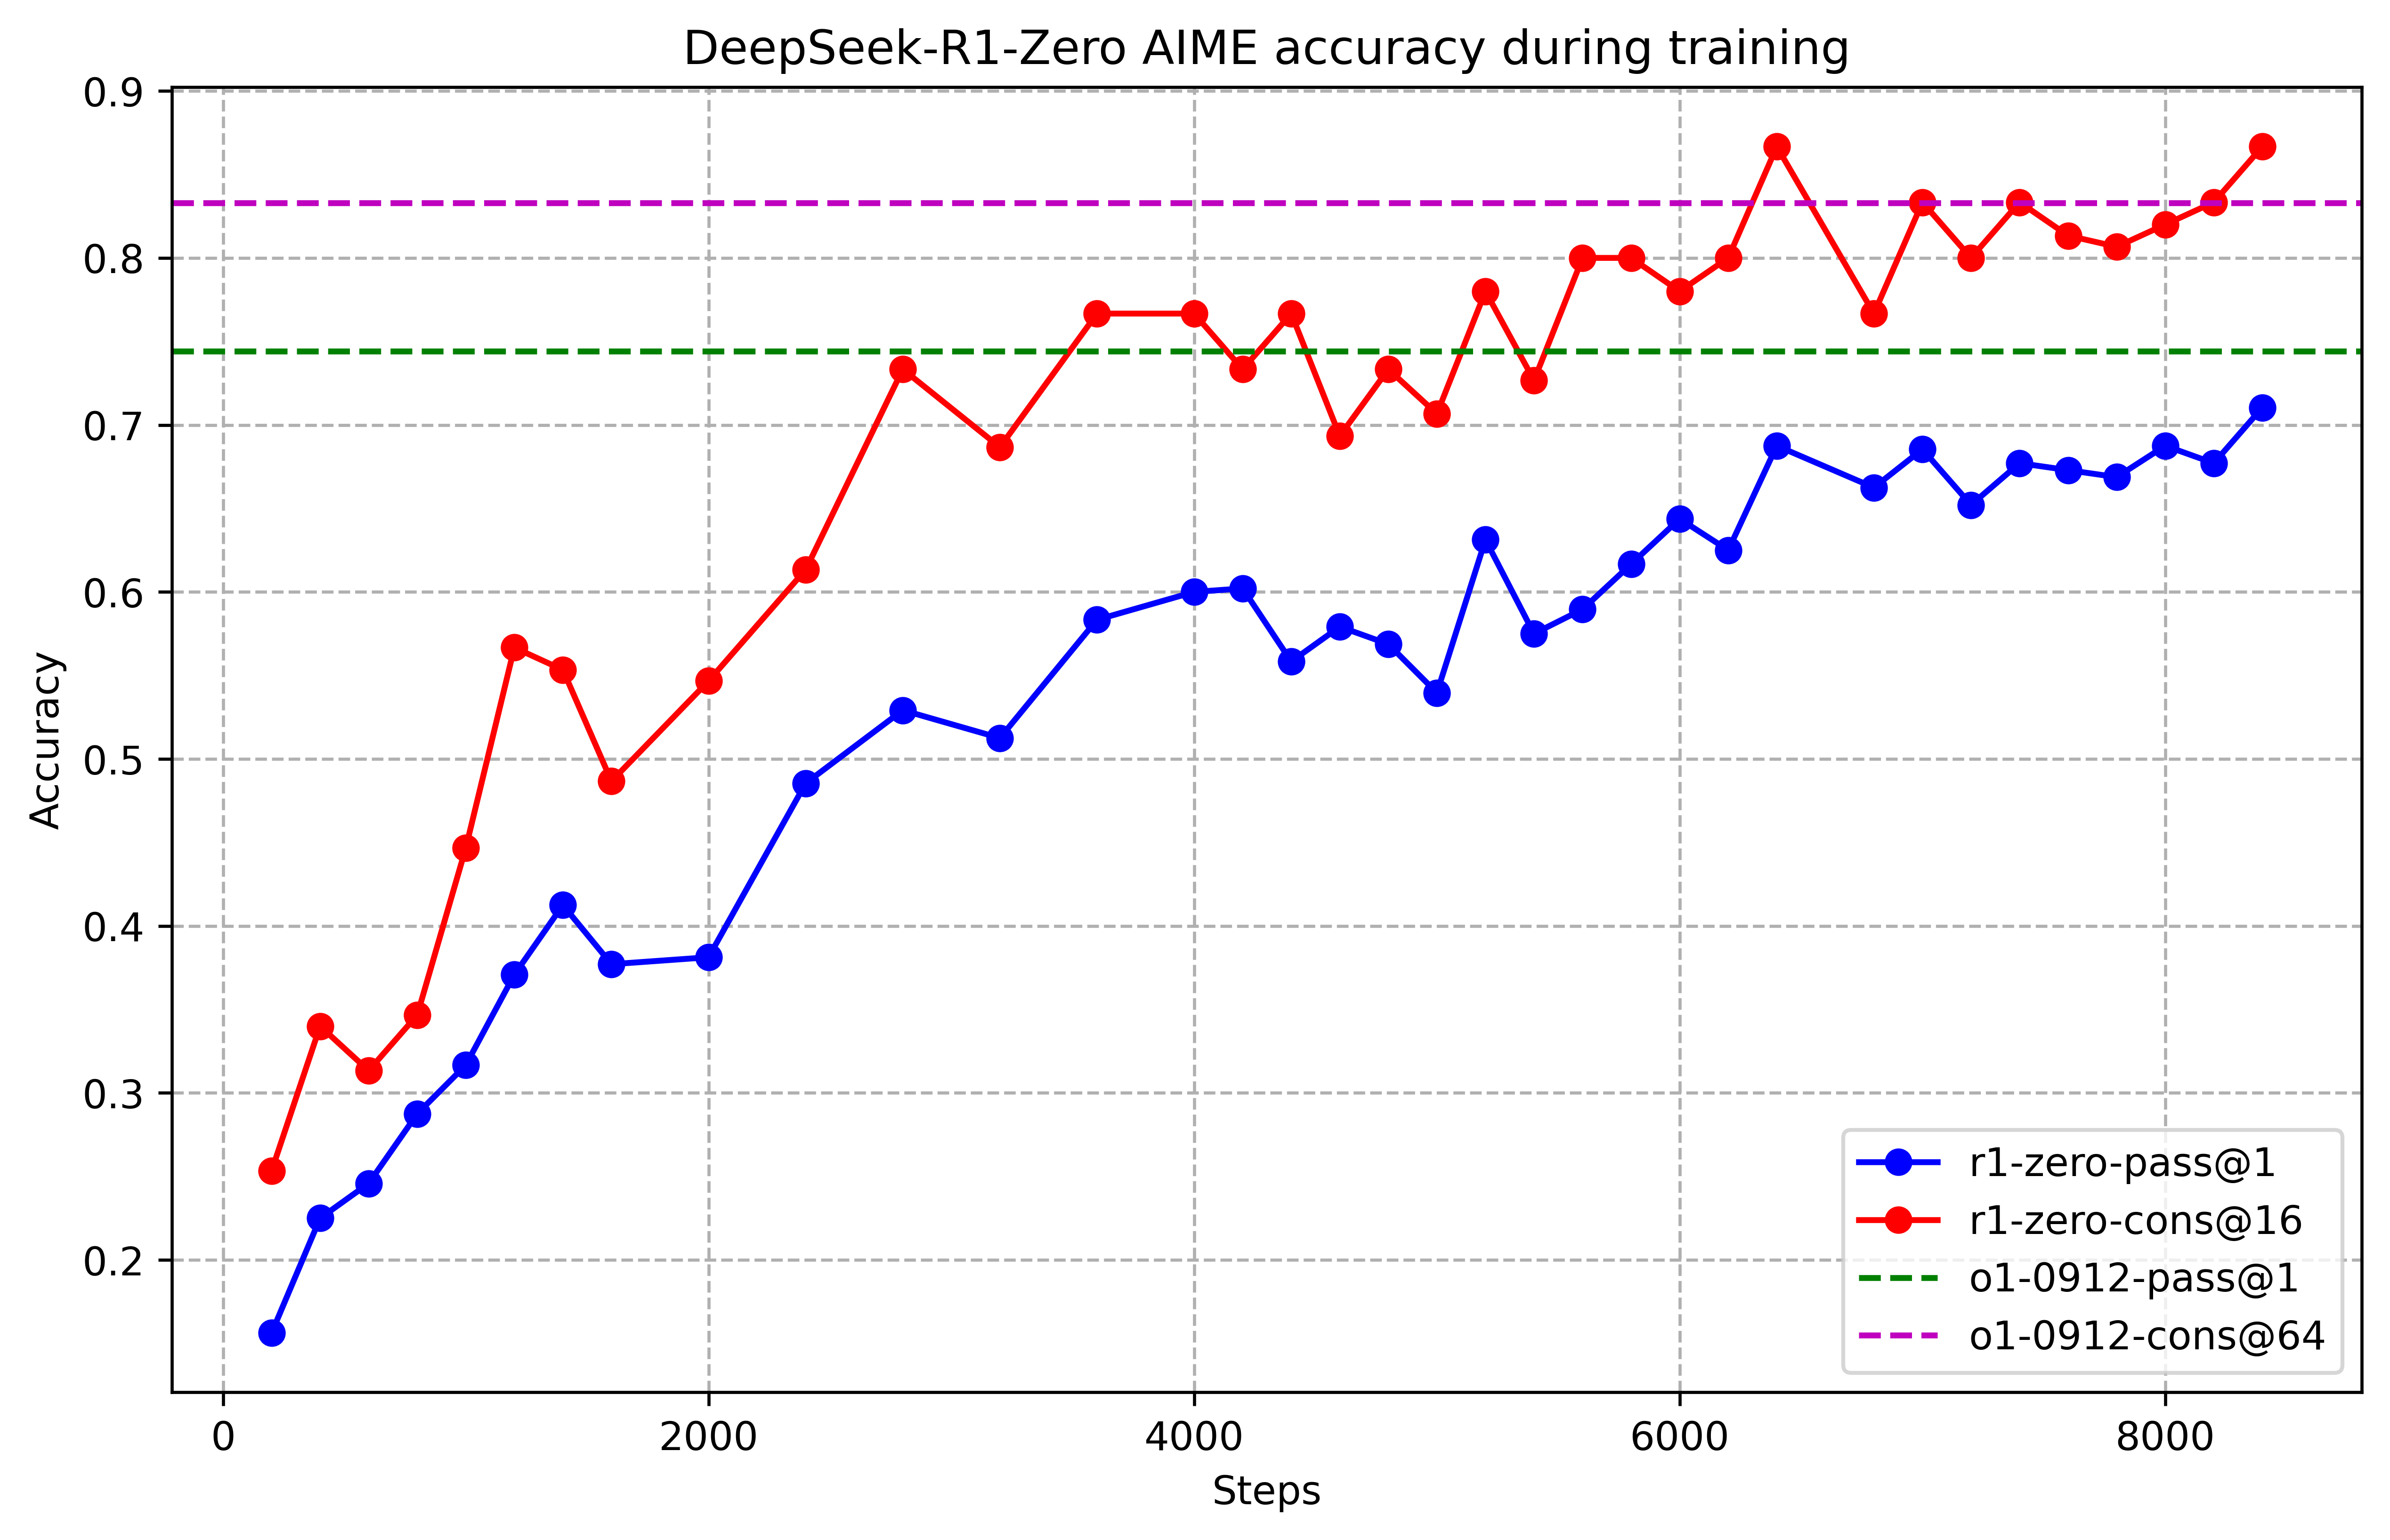
\includegraphics[width=0.75\linewidth]{figures/plot_aime_with_maj.png}
  \caption{\dsro{} 的训练过程中,在 AIME 上的准确性。针对每个问题,我们采样 16 个响应并计算平均准确性,来保证稳定的评估。}
  \label{fig:zero-training-performance}
\end{figure}

图 \ref{fig:zero-training-performance} 展示了 \dsro{} 在 AIME 2024 基准测试中整个强化学习训练过程中的性能轨迹。如图所示,随着强化学习训练的推进,\dsro{} 的性能稳步而持续地提升。值得注意的是,AIME 2024 上的平均 pass@1 分数显著增加,从最初的 15.6\% 跃升至令人印象深刻的 71.0\%,达到了与 OpenAI-o1-0912 相当的性能水平。这一显著的改进突显了我们强化学习算法在优化模型性能方面的有效性。

表 \ref{tab:r1-zero} 提供了 \dsro{} 与 OpenAI 的 o1-0912 模型在各种推理相关基准测试中的比较分析。研究结果显示,强化学习使 \dsro{} 能够在没有任何监督微调数据的情况下获得强大的推理能力。这是一个值得注意的成就,因为它强调了模型仅通过强化学习就能有效学习和泛化的能力。此外,通过使用多数投票,\dsro{} 的性能可以进一步增强。例如,当在 AIME 基准上使用多数投票时,\dsro{} 的性能从 71.0\% 提升至 86.7\%,从而超越了 OpenAI-o1-0912 的性能。\dsro{} 在有无多数投票的情况下都能实现如此具有竞争力的性能,突显了其强大的基础能力以及在推理任务中进一步发展的潜力。

\begin{figure}[t]
  \centering
  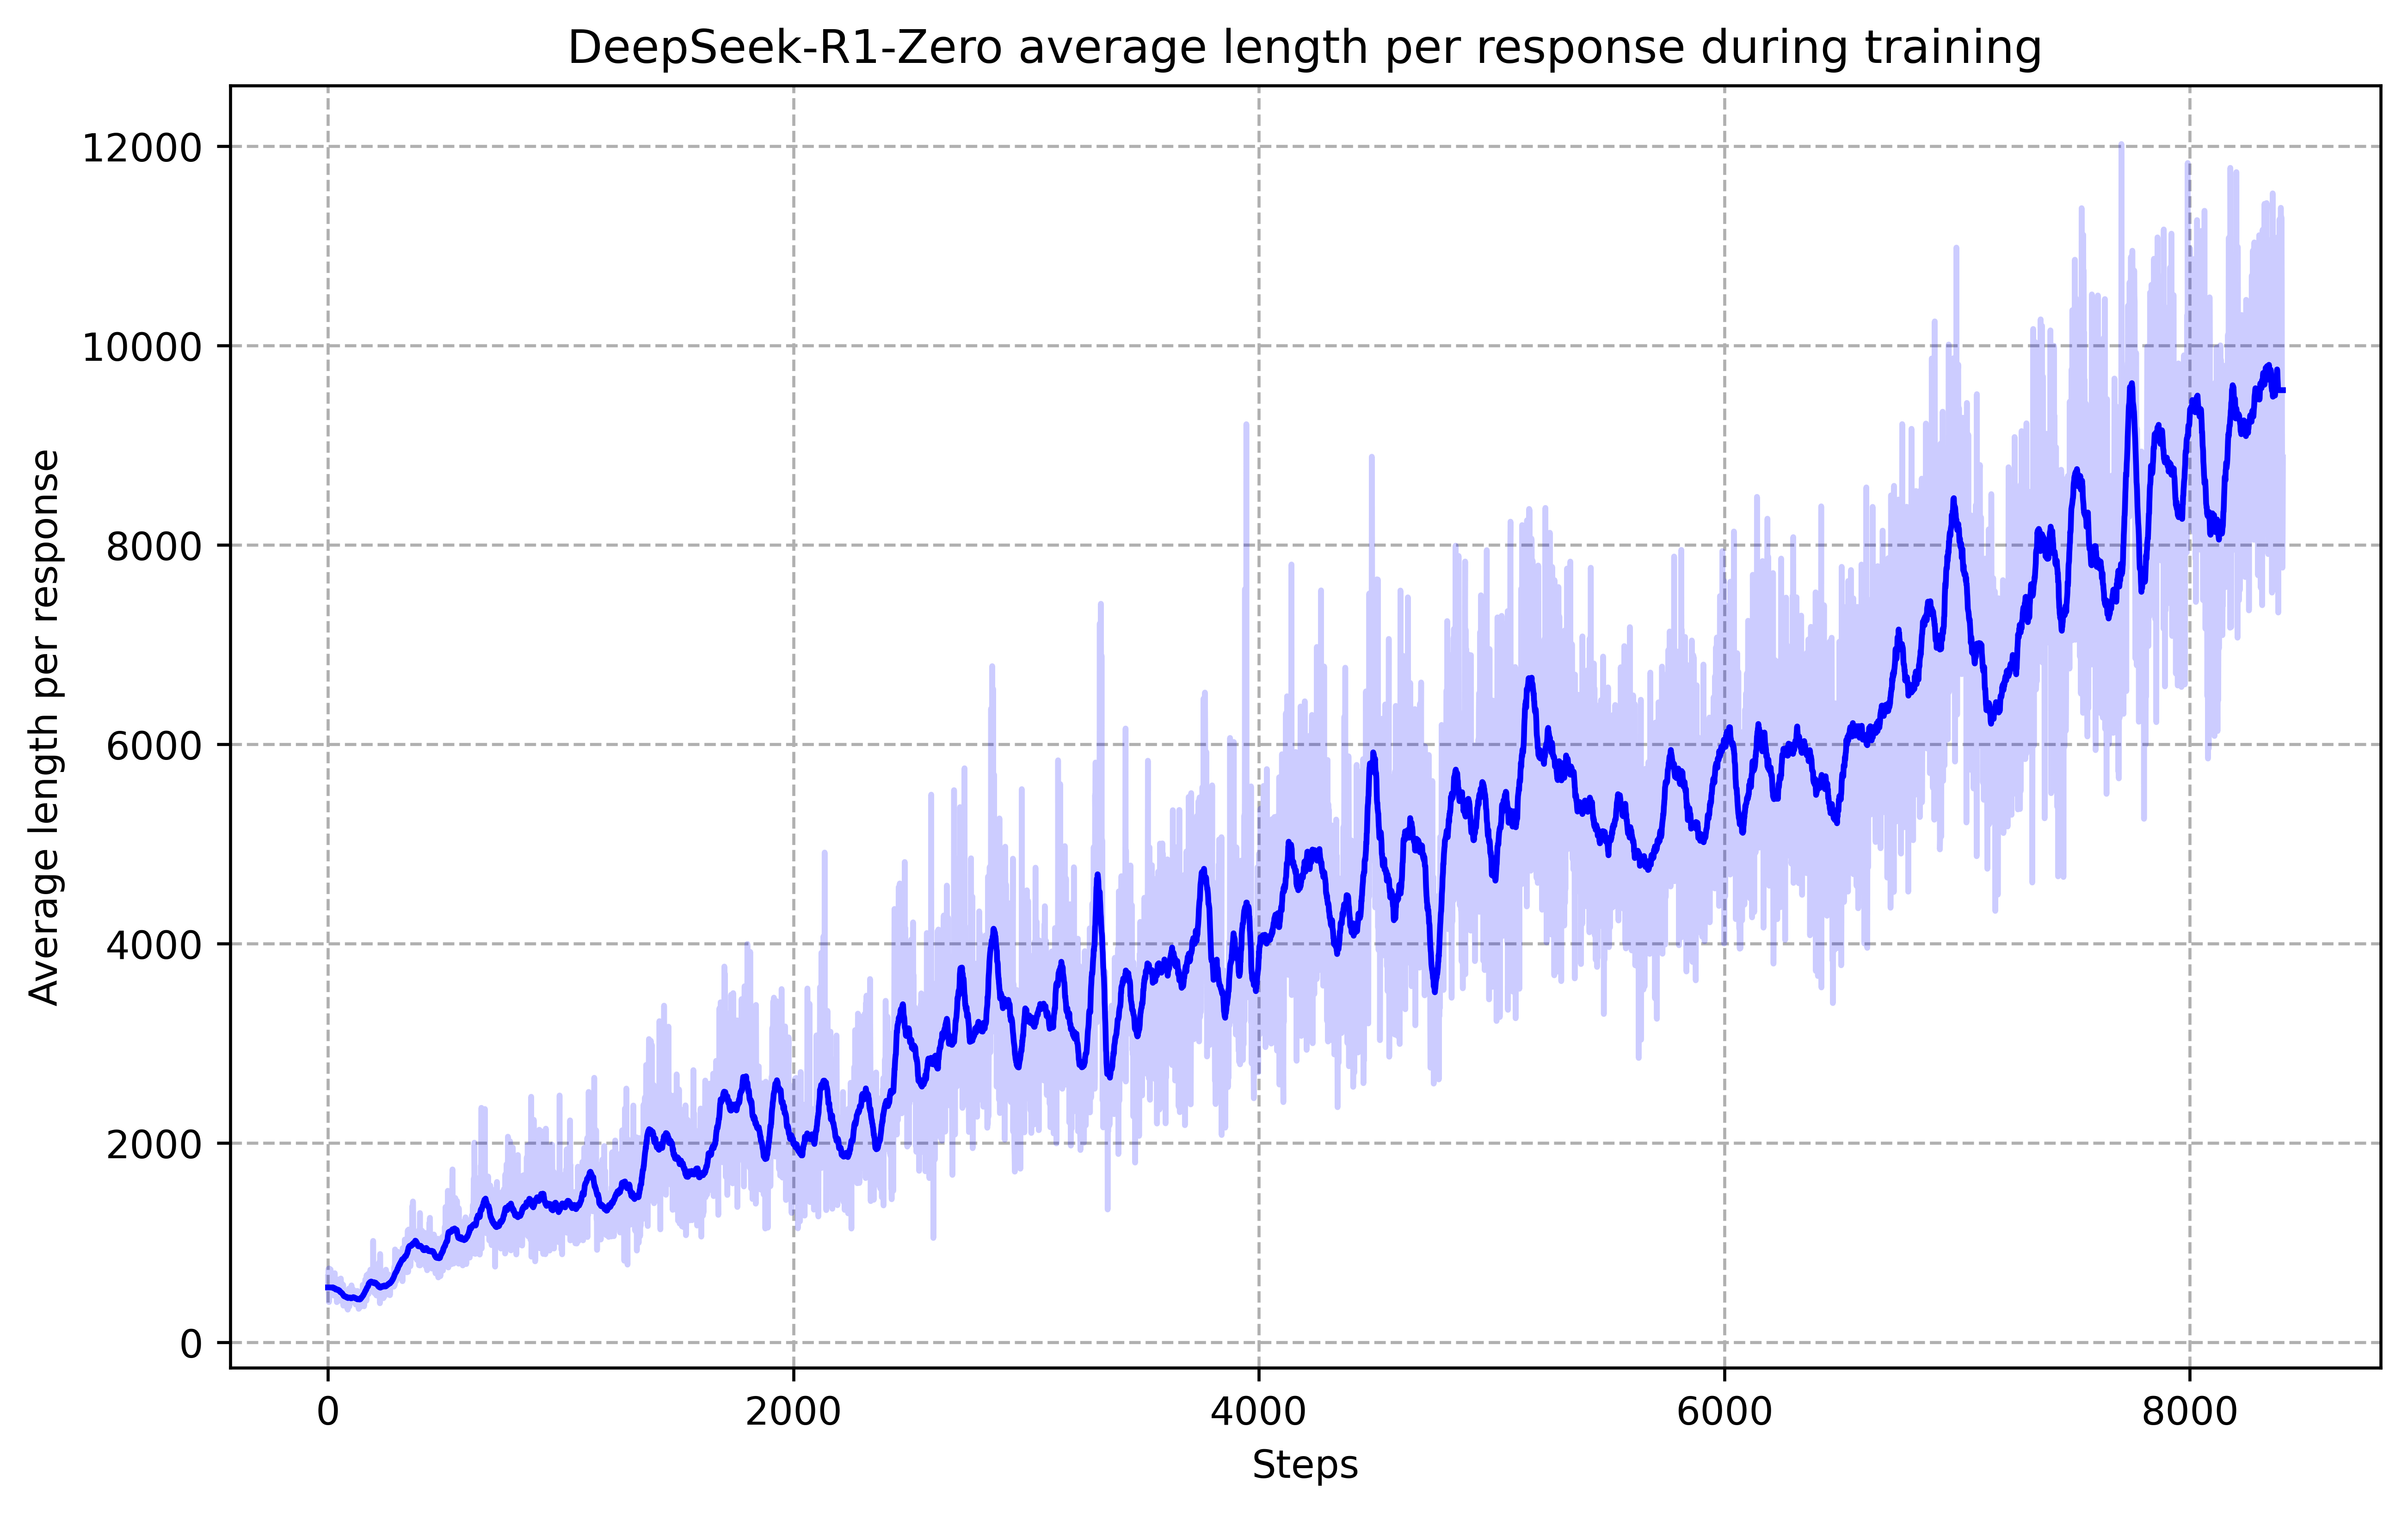
\includegraphics[width=0.75\linewidth]{figures/plot_length.png}
  \caption{在强化学习过程中,\dsro{} 在训练集上响应的平均长度。\dsro{} 通过更多的思考时间自己学会了解决推理任务。}
  \label{fig:zero-training-length}
\end{figure}

\paragraph{\dsro{} 的自我进化过程}

\dsro{} 的自我进化过程是一个引人入胜的示例,展示了强化学习如何驱动模型自主提升其推理能力。通过直接从基础模型启动强化学习,我们可以在没有监督微调阶段影响的情况下,密切监控模型的进展。这种方法清晰地展示了模型随时间演变的过程,特别是在处理复杂推理任务的能力方面。

如图 \ref{fig:zero-training-length} 所示,\dsro{} 的思考时间在整个训练过程中持续改善。这种改善并不是外部调整的结果,而是模型内部的内在发展。通过利用延长的测试时间计算,\dsro{} 自然获得了解决日益复杂的推理任务的能力。这种计算范围从生成数百到数千个推理标记,使模型能够更深入地探索和完善其思考过程。

这一自我进化过程中最显著的一个方面是,随着测试时间计算的增加,复杂行为的出现。例如,反思行为——模型重新审视和重新评估其之前的步骤——以及探索替代问题解决方法的能力自发地产生。这些行为并不是显式编程的,而是模型与强化学习环境互动的结果。这种自发的发展显著增强了 \dsro{} 的推理能力,使其能够更高效、更准确地应对更具挑战性的任务。

\paragraph{\dsro{} 的“顿悟”时刻}

在 \dsro{} 的训练过程中观察到的一个特别引人入胜的现象是“顿悟”时刻的出现。如表 \ref{tab:aha_moment} 所示,这一时刻发生在模型的一个中间版本中。在这一阶段,\dsro{} 学会通过重新评估其初始方法来为问题分配更多的思考时间。这种行为不仅证明了模型推理能力的提升,也是强化学习如何导致意想不到且复杂结果的迷人示例。

这一时刻不仅是模型的“顿悟”时刻,也是观察其行为的研究人员的“顿悟”时刻。它突显了强化学习的力量和美妙:我们并不是明确教导模型如何解决问题,而是简单地为其提供正确的激励,模型便能自主发展出先进的问题解决策略。“顿悟”时刻强有力地提醒我们,强化学习有潜力在人工系统中开启新的智能水平,为未来更自主和适应性强的模型铺平道路。

\paragraph{\dsro{} 的缺陷}

尽管 \dsro{} 展示了强大的推理能力,并自主发展出意想不到且强大的推理行为,但它仍面临一些问题。例如,\dsro{} 在可读性差和多语言混合等挑战上存在困难。为了使推理过程更加可读并与开放社区分享,我们探索了 \dsri{},这是一种利用人类友好的冷启动数据的强化学习方法。

\begin{table}[t]
  \centering
  \begin{tabular}{l}
  \toprule 
  问题: 如果 \(a > 1\), 则方程 \(\sqrt{a - \sqrt{a + x}} = x\) 的实数解的和等于 \\
  \midrule
  响应: <think> \\
  为了解方程 \(\sqrt{a - \sqrt{a + x}} = x\), 让我们首先将等式两边进行平方 $\cdots$ \\
  $\left(\sqrt{a - \sqrt{a + x}}\right)^2 = x^2 \implies a - \sqrt{a + x} = x^2.$ \\
  通过移项将根号中的表达式独立出来: \\
  $(a - x^2)^2 = a + x \implies a^2 - 2ax^2 + (x^2)^2 = a + x \implies x^4 - 2ax^2 - x + (a^2 - a) = 0$ \\
  \ldots \\
  \textcolor{red}{等一下, 等一下, 等一下。这是个顿悟时刻, 我要记一下.}. \\
  让我们一步一步重新求值来检查一下正确的和是否是 $\cdots$ \\
  我们先从下面的等式开始: \\
  $\sqrt{a - \sqrt{a + x}} = x$ \\
  首先,让我们先将等式两边平方: \\
  $a - \sqrt{a + x} = x^2 \implies \sqrt{a + x} = a - x^2$ \\
  接下来, 我可以再将等式两边平方, 然后处理以下等式: 
  $\cdots$
  \\
  \ldots \\
  \hline
  \end{tabular}
  \caption{\dsro{}中间版本的一个有趣的“顿悟”时刻。模型学会了以拟人化的语气进行重新思考。这对我们来说也是一个顿悟时刻,让我们见证了强化学习的力量与美感。}
  \label{tab:aha_moment}
  \end{table}

\subsection{\dsri{}:带冷启动的强化学习}

受到 \dsro{} 令人鼓舞的结果启发,产生了两个自然的问题:

\begin{enumerate}
  \item 是否可以通过引入少量高质量数据作为冷启动,进一步提高推理性能或加速收敛?
  \item 我们如何训练一个用户友好的模型,使其不仅能生成清晰连贯的思维链(CoT),还能够展现出强大的通用能力?
\end{enumerate}

为了解决这些问题,我们设计了一个训练 \dsri{} 的流程。该流程由四个阶段组成,具体如下。

\subsubsection{冷启动}

与 \dsro{} 不同,为了防止基础模型在强化学习训练的早期处于不稳定的冷启动阶段,对于 DeepSeek-R1,我们构建并收集了一小部分思维链(CoT)数据,来把模型微调成最初的强化学习演员。

为了收集这些数据,我们探索了几种方法:使用长思维链推理作为示例的少量提示,直接提示模型生成详细的答案并进行反思和验证,以人类可读的格式来收集 \dsro{} 的输出,以及通过人工标注者对结果进行后处理和精炼。

在这项工作中,我们收集了数千条冷启动数据,将 DeepSeek-V3-Base 微调成强化学习的起点。与 \dsro{} 相比,冷启动数据的优势包括:

\begin{itemize}[topsep=0pt]
  \item 可读性:\dsro{} 的一个主要限制是其内容通常不适合人类阅读。响应可能混合多种语言,或者缺乏 markdown 格式来突出显示用户的答案。相比之下,在为 \dsri{} 创建冷启动数据时,我们设计了一种可读的模式,包括每个响应末尾的摘要,并过滤掉不适合阅读的响应。在这里,我们将输出格式定义为 |special\_token|<reasoning\_process>|special\_token|<summary>,其中推理过程是针对查询的思维链(CoT),摘要用于总结推理结果。
  \item 潜力:通过精心设计带有人类先验的冷启动数据模式,我们观察到相较于 \dsro{} 更好的性能。我们相信,迭代训练是推理模型更好的方法。
\end{itemize}

\subsubsection{推理导向的强化学习}

在使用冷启动数据对 DeepSeek-V3-Base 进行微调后,我们应用与 \dsro{} 模型相同的大规模强化学习训练过程。此阶段重点提升模型的推理能力,特别是在编码、数学、科学和逻辑推理等推理密集型任务中,这些任务涉及明确定义的问题和清晰的解决方案。在训练过程中,我们观察到思维链(CoT)常常表现出多种语言的混合,尤其是在强化学习提示涉及多种语言时。为了缓解语言混合的问题,我们在强化学习训练中引入了语言一致性奖励,该奖励计算思维链中目标语言单词的比例。尽管消融实验表明,这种对齐会导致模型性能的轻微下降,但该奖励与人类偏好一致,使其更具可读性。最后,我们通过直接相加推理任务的准确性和语言一致性奖励来形成最终奖励。然后,我们在微调后的模型上进行强化学习训练,直到其在推理任务上达到收敛。

\subsubsection{拒绝采样和监督微调}

当面向推理的强化学习收敛时,我们利用生成的检查点收集后续轮次的监督微调(SFT)数据。与最初主要关注推理的冷启动数据不同,此阶段纳入了来自其他领域的数据,以增强模型在写作、角色扮演和其他通用任务中的能力。具体而言,我们生成数据并按以下方式微调模型。
\label{sec:method:r1:sft}

\paragraph{推理数据}
我们策划推理提示,并通过对上述强化学习训练的检查点进行拒绝采样来生成推理轨迹。在前一个阶段,我们只包含了可以通过基于规则的奖励进行评估的数据。然而,在这一阶段,我们通过纳入额外的数据来扩展数据集,其中一些数据使用生成奖励模型,通过将真实答案和模型预测输入 DeepSeek-V3 进行判断。

此外,由于模型输出有时混乱且难以阅读,我们过滤掉了包含混合语言、长段落和代码块的链推理。对于每个提示,我们采样多个响应,仅保留正确的响应。总共,我们收集了大约 60 万个与推理相关的训练样本。

\paragraph{无推理数据}
对于非推理类数据,例如写作、事实问答、自我认知和翻译,我们采用DeepSeek-V3的流程,并复用部分DeepSeek-V3的监督微调数据集。对于某些非推理任务,我们会调用DeepSeek-V3生成潜在的思维链,然后再通过提示回答问题。然而,对于较简单的查询,例如“你好”,我们不会在响应中提供思维链。

最终,我们收集了大约20万个与推理无关的训练样本。

我们使用上述约80万个样本的数据集对DeepSeek-V3-Base进行了两个周期的微调。

\subsubsection{针对所有场景的强化学习}

为了进一步使模型与人类偏好对齐,我们实施了第二阶段的强化学习,旨在提高模型的有用性和无害性,同时增强其推理能力。具体来说,我们结合奖励信号和多样化的提示分布来训练模型。

对于推理类数据,我们遵循了\dsro{} 中概述的方法,该方法利用基于规则的奖励来指导数学、代码和逻辑推理领域的学习过程。

对于通用数据,我们采用奖励模型来捕捉复杂和微妙场景中的人类偏好。我们在DeepSeek-V3流程的基础上,采用了类似的偏好对和训练提示分布。在有用性方面,我们专注于最终总结,确保评估强调响应对用户的实用性和相关性,同时尽量减少对底层推理过程的干扰。在无害性方面,我们评估模型的整个响应,包括推理过程和总结,以识别并减轻生成过程中可能出现的任何潜在风险、偏见或有害内容。

最终,通过整合奖励信号和多样化的数据分布,我们能够训练出一个在推理方面表现出色,同时优先考虑有用性和无害性的模型。

\subsection{蒸馏:为小模型赋能推理能力}

为了让更高效的小模型像\dsri{}具备推理能力,我们直接使用\dsri{}整理的80万个样本对开源模型(如Qwen和Llama)进行了微调,具体细节见\S \ref{sec:method:r1:sft}。

我们的研究结果表明,这种直接的蒸馏方法显著提升了小模型的推理能力。我们使用的基础模型包括Qwen2.5-Math-1.5B、Qwen2.5-Math-7B、Qwen2.5-14B、Qwen2.5-32B、Llama-3.1-8B和Llama-3.3-70B-Instruct。我们选择Llama-3.3是因为其推理能力略优于Llama-3.1。

对于蒸馏后的模型,我们仅使用了监督微调,并未加入强化学习阶段,尽管引入强化学习可以显著提升模型性能。我们的主要目标是展示蒸馏技术的有效性,而将强化学习阶段的探索留给更广泛的研究社区。

\section{实验}

\paragraph{基准测试} 我们在以下基准上评估模型:MMLU、MMLU-Redux、MMLU-Pro、C-Eval、CMMLU、IFEval、FRAMES、GPQA Diamond、SimpleQA、C-SimpleQA、SWE-Bench Verified、Aider、LiveCodeBench、Codeforces、中国高中数学奥林匹克(CNMO 2024)以及美国数学邀请赛2024(AIME 2024)。

除了标准基准测试外,我们还使用大语言模型作为评判者对开放式生成任务进行评估。具体来说,我们遵循AlpacaEval 2.0和Arena-Hard的原始配置,利用GPT-4-Turbo-1106作为评判者进行成对比较。在这里,我们仅将最终总结提供给评估,以避免长度偏差。

对于蒸馏模型,我们报告了在AIME 2024、MATH-500、GPQA Diamond、Codeforces和LiveCodeBench上的代表性结果。

\paragraph{评估提示} 遵循DeepSeek-V3的设置,标准基准测试(如MMLU、DROP、GPQA Diamond和SimpleQA)使用simple-evals框架中的提示进行评估。对于MMLU-Redux,我们采用Zero-Eval提示格式,并在零样本设置下进行评估。对于MMLU-Pro、C-Eval和CLUE-WSC,由于原始提示是少样本的,我们略微修改了提示以适应零样本设置。少样本中的思维链(CoT)可能会影响\dsri{}的性能。

其他数据集遵循其原始评估协议,并使用其创建者提供的默认提示。对于代码和数学基准测试,HumanEval-Mul数据集涵盖了八种主流编程语言(Python、Java、C++、C\#、JavaScript、TypeScript、PHP和Bash)。LiveCodeBench上的模型性能使用思维链(CoT)格式进行评估,数据收集时间为2024年8月至2025年1月。Codeforces数据集使用10场Div.2比赛的题目以及专家编写的测试用例进行评估,随后计算预期评分和参赛者百分比。SWE-Bench的验证结果通过无代理框架获得。AIDER相关基准测试使用“diff”格式进行测量。

\dsri{}的输出在每个基准测试中最多限制为32,768个token。

\paragraph{基线模型} 我们对多个强基线模型进行了全面评估,包括DeepSeek-V3、Claude-Sonnet-3.5-1022、GPT-4o-0513、OpenAI-o1-mini和OpenAI-o1-1217。由于在中国大陆访问OpenAI-o1-1217的API较为困难,我们根据官方报告记录了其性能。

对于蒸馏模型,我们还比较了开源模型QwQ-32B-Preview。

\paragraph{评估设置}  
我们将模型的最大生成长度设置为32,768个token。我们发现,使用贪心解码来评估长输出推理模型会导致更高的重复率,并且不同检查点之间的变异性较大。因此,我们默认使用pass@$k$评估方法,并在非零温度下报告pass@1。具体来说,我们使用采样温度为$0.6$,top-$p$值为$0.95$,为每个问题生成$k$个响应(通常在$4$到$64$之间,取决于测试集大小)。然后,pass@1的计算公式为:
\[
\text{pass@1} = \frac{1}{k} \sum_{i=1}^{k} p_i,
\]
其中$p_i$表示第$i$个响应的正确性。这种方法提供了更可靠的性能估计。对于AIME 2024,我们还报告了使用$64$个样本的共识(多数投票)结果,记为$\text{cons}@64$。

\subsection{\dsri{} 的评估}
\begin{table}[h]
    \centering
    \footnotesize
    \setlength{\tabcolsep}{1.9pt}
    \begin{tabular}{@{}c l | c  c  c | c c |c c@{}}
    \toprule
    & \multirow{2}{*}{\centering \textbf{Benchmark {\tiny (Metric)}}}  & \textbf{Claude-3.5-}  & \textbf{GPT-4o}& \textbf{DeepSeek} & \textbf{OpenAI} & \textbf{OpenAI} & \textbf{DeepSeek}\\
    & & \textbf{Sonnet-1022}  & \textbf{0513} & \textbf{V3} & \textbf{o1-mini}& \textbf{o1-1217} &\textbf{R1} \\
    \midrule
    & Architecture &-&- & MoE &-&-& MoE \\
    & \# Activated Params& -&-& 37B&-&- & 37B \\
    & \# Total Params &-&-& 671B&-&- & 671B \\
    \midrule
    \multirow{10}{*}{English}& MMLU {\tiny (Pass@1)} & 88.3&87.2 & 88.5 & 85.2 & \textbf{91.8} & 90.8\\
     & MMLU-Redux {\tiny (EM)}& 88.9& 88.0 & 89.1 & 86.7&- & \textbf{92.9} \\
    & MMLU-Pro {\tiny (EM)}  & 78.0 & 72.6 & 75.9 & 80.3 &-& \textbf{84.0} \\
    & DROP {\tiny (3-shot F1)}  & 88.3 & 83.7 & 91.6 & 83.9 & 90.2 & \textbf{92.2}\\
    & IF-Eval {\tiny (Prompt Strict)}  & \textbf{86.5} & 84.3 & 86.1 & 84.8&- & 83.3 \\
    & GPQA Diamond {\tiny (Pass@1)}& 65.0 & 49.9 & 59.1 & 60.0 & \textbf{75.7} & 71.5&  \\
    & SimpleQA {\tiny (Correct)} & 28.4 & 38.2& 24.9 & 7.0 & \textbf{47.0} & 30.1 \\
     & FRAMES {\tiny (Acc.)}  & 72.5 & 80.5 & 73.3 & 76.9 & -&\textbf{82.5}\\
      & AlpacaEval2.0 {\tiny (LC-winrate)}  & 52.0 &  51.1 & 70.0 & 57.8 & - & \textbf{87.6}\\
       & ArenaHard {\tiny (GPT-4-1106)}  & 85.2 & 80.4 & 85.5 & 92.0 & - & \textbf{92.3}\\
    \midrule
    \multirow{4}{*}{Code} & LiveCodeBench {\tiny (Pass@1-COT)} & 38.9 & 32.9 & 36.2 & 53.8 & 63.4 & \textbf{65.9} \\
    & Codeforces {\tiny (Percentile)}& 20.3 & 23.6 & 58.7 & 93.4 & \textbf{96.6} & 96.3 \\
    & Codeforces {\tiny (Rating)}& 717 & 759 & 1134 & 1820 & \textbf{2061} & 2029 \\
    & SWE Verified {\tiny (Resolved)} & \textbf{50.8}&38.8&42.0 & 41.6 & 48.9 & 49.2\\
    & Aider-Polyglot {\tiny (Acc.)} & 45.3&16.0& 49.6 & 32.9 & \textbf{61.7}&53.3\\
    \midrule
    \multirow{3}{*}{Math} & AIME 2024 {\tiny (Pass@1)}  & 16.0 & 9.3 & 39.2 & 63.6 & 79.2 & \textbf{79.8} \\
    & MATH-500 {\tiny (Pass@1)} &78.3 & 74.6&90.2 & 90.0 & 96.4 & \textbf{97.3} \\
    & CNMO 2024 {\tiny (Pass@1)} & 13.1 & 10.8 &43.2 & 67.6 & - & \textbf{78.8} \\
    \midrule
    \multirow{3}{*}{Chinese} & CLUEWSC {\tiny (EM)}&  85.4 & 87.9 & 90.9 & 89.9 & - &\textbf{92.8}\\
    & C-Eval {\tiny (EM)} & 76.7 & 76.0 & 86.5 & 68.9 & - & \textbf{91.8}\\
     & C-SimpleQA {\tiny (Correct)}  & 55.4 & 58.7 & \textbf{68.0} & 40.3 & -& 63.7 \\
    \bottomrule
    \end{tabular}
    \caption{ \dsri{} 与其他代表性模型的比较。 }
    \label{tab:main}
\end{table}


对于教育导向的知识基准测试,例如 MMLU、MMLU-Pro 和 GPQA Diamond,\dsri{} 相较于 DeepSeek-V3 展现出更优越的表现。这一改进主要归因于在 STEM 相关问题上的准确性提升,通过大规模强化学习取得了显著的进展。此外,\dsri{} 在 FRAMES 这一长上下文依赖的问答任务上表现出色,展现了其强大的文档分析能力。这突显了推理模型在 AI 驱动的搜索和数据分析任务中的潜力。在事实基准测试 SimpleQA 上,\dsri{} 超越了 DeepSeek-V3,展示了其处理基于事实的查询的能力。在这一基准测试中,OpenAI-o1 也超越了 GPT-4o。然而,\dsri{} 在中文 SimpleQA 基准测试中的表现逊色于 DeepSeek-V3,主要是因为其在安全强化学习后倾向于拒绝回答某些查询。如果没有安全强化学习,\dsri{} 的准确率可以超过 70%。

\dsri{} 在 IF-Eval 上也取得了令人印象深刻的结果,该基准旨在评估模型遵循格式指令的能力。这些改进与在监督微调(SFT)和强化学习训练的最后阶段纳入指令遵循数据有关。此外,在 AlpacaEval2.0 和 ArenaHard 上也观察到了显著的表现,表明 \dsri{} 在写作任务和开放域问答方面的优势。它显著超越 DeepSeek-V3 的表现强调了大规模强化学习的泛化优势,这不仅提升了推理能力,还改善了在多种领域的表现。

此外,\dsri{} 生成的摘要长度简洁,在 ArenaHard 上平均为 689 个 token,在 AlpacaEval 2.0 上为 2,218 个字符。这表明 \dsri{} 在基于 GPT 的评估中避免了引入长度偏差,进一步巩固了其在多个任务中的鲁棒性。

在数学任务上,\dsri{} 的表现与 OpenAI-o1-1217 相当,远超其他模型。在编码算法任务上,如 LiveCodeBench 和 Codeforces,也观察到了类似的趋势,推理为重点的模型在这些基准测试中占据主导地位。在工程导向的编码任务中,OpenAI-o1-1217 在 Aider 上超越了 \dsri{},但在 SWE Verified 上的表现相当。我们相信,\dsri{} 在下一版本中的工程性能将有所提升,因为目前相关的强化学习训练数据仍然非常有限。

\subsection{蒸馏模型的评估}
\label{sec:distilled_model_evaluation}
\begin{table}[h]
    \centering
    \resizebox{\linewidth}{!}{
    \begin{tabular}{@{}l *{6}{c} @{}}
    \toprule
    \multirow{3}{*}{\centering\textbf{Model}} & \multicolumn{2}{c}{\multirow{2}{*}{\textbf{AIME 2024}}} & \multirow{2}{*}{\textbf{MATH-500}} & \textbf{GPQA} & \textbf{LiveCode} & \multirow{2}{*}{\textbf{CodeForces}} \\
    &  &  &  & \textbf{Diamond} & \textbf{Bench} \\
    \cmidrule(lr){2-3}
     & pass@1 & cons@64 & pass@1 & pass@1 & pass@1 & rating \\
    \midrule
    \textbf{GPT-4o-0513} & 9.3 & 13.4 & 74.6  & 49.9 & 32.9 &  759\\
    \textbf{Claude-3.5-Sonnet-1022} & 16.0 & 26.7 & 78.3  & 65.0 & 38.9 &  717\\
    \textbf{OpenAI-o1-mini} & 63.6 & 80.0 & 90.0 &  60.0 & 53.8 &  \textbf{1820}\\
    \textbf{QwQ-32B-Preview} & 50.0 & 60.0 & 90.6 & 54.5 & 41.9 &  1316 \\
    \midrule
    \textbf{DeepSeek-R1-Distill-Qwen-1.5B} & 28.9 & 52.7 & 83.9 & 33.8 & 16.9 & 954 \\
    \textbf{DeepSeek-R1-Distill-Qwen-7B} & 55.5 & 83.3 & 92.8 & 49.1 & 37.6 & 1189 \\
    \textbf{DeepSeek-R1-Distill-Qwen-14B} & 69.7 & 80.0 & 93.9 &  59.1 & 53.1 & 1481 \\
    \textbf{DeepSeek-R1-Distill-Qwen-32B} & \textbf{72.6} & {83.3} & {94.3} & {62.1} & {57.2} & 1691 \\
    \textbf{DeepSeek-R1-Distill-Llama-8B} & 50.4 & 80.0 & 89.1 & 49.0 & 39.6 & 1205 \\
    \textbf{DeepSeek-R1-Distill-Llama-70B} & 70.0 & \textbf{86.7} & \textbf{94.5} & \textbf{65.2} & \textbf{57.5} & 1633 \\
    \bottomrule
    \end{tabular}
    }
    \caption{经过 DeepSeek-R1 蒸馏过的模型和其它类似的模型在推理相关任务上的基准测试。}
    \label{tab:distill}
\end{table}



如表 \ref{tab:distill} 所示,简单地使用 DeepSeek-R1 的输出来蒸馏 DeepSeek-R1-7B ,使得高效的 DeepSeek-R1-7B(即 DeepSeek-R1-Distill-Qwen-7B,以下简写相同)在各方面超越了像 GPT-4o-0513 这样的非推理模型。DeepSeek-R1-14B 在所有评估指标上超过了 QwQ-32B-Preview,而 DeepSeek-R1-32B 和 DeepSeek-R1-70B 在大多数基准测试中显著超过了 o1-mini。这些结果展示了蒸馏的强大潜力。此外,我们发现将强化学习应用于这些蒸馏模型可以带来显著的进一步提升。我们认为这值得进一步探索,因此在此仅展示简单的通过监督微调来蒸馏模型的结果。

\section{讨论}

\subsection{蒸馏 v.s. 强化学习}

\begin{table}[h]
    \centering
    \resizebox{\linewidth}{!}{
    \begin{tabular}{@{}l *{6}{c} @{}}
    \toprule
    \multirow{3}{*}{\centering\textbf{Model}} & \multicolumn{2}{c}{\textbf{AIME 2024}} & \textbf{MATH-500} & \textbf{GPQA Diamond} & \textbf{LiveCodeBench}  \\

    \cmidrule(lr){2-3}
     & pass@1 & cons@64 & pass@1& pass@1 & pass@1 \\
    \midrule
    \textbf{QwQ-32B-Preview} & 50.0 & 60.0 & 90.6 & 54.5 & 41.9  \\
    \textbf{DeepSeek-R1-Zero-Qwen-32B} & 47.0 & 60.0 & 91.6  & 55.0 & 40.2  \\
    \textbf{DeepSeek-R1-Distill-Qwen-32B} & \bf{72.6} & \bf{83.3} & \bf{94.3}  & \bf{62.1} & \bf{57.2}\\
    \bottomrule
    \end{tabular}
    }
    \caption{\centering 推理相关基准测试中,经过蒸馏的小模型和经过强化学习的小模型的性能比较。}
    \label{tab:distill_vs_rl}
\end{table}


在第 \ref{sec:distilled_model_evaluation} 节中,我们可以看到,通过使用 DeepSeek-R1 的输出对小模型进行蒸馏,小模型能够取得令人印象深刻的结果。然而,仍然有一个问题:模型是否可以通过本文讨论的大规模强化学习训练而不进行蒸馏来实现可比的性能?

为了解答这个问题,我们在 Qwen-32B-Base 上进行了大规模强化学习训练,使用数学、代码和 STEM 数据,训练超过 10K 步,最终得到了 \dsro{}-Qwen-32B。实验结果如表 \ref{tab:distill_vs_rl} 所示,经过大规模强化学习训练后,32B 基础模型的性能与 QwQ-32B-Preview 相当。然而,从 DeepSeek-R1 蒸馏而来的 DeepSeek-R1-Distill-Qwen-32B 在所有基准测试中表现显著优于 \dsro{}-Qwen-32B。

因此,我们可以得出两个结论:首先,将更强大的模型蒸馏为更小的模型能够获得优异的结果,而依赖于本文提到的大规模强化学习的小模型则需要巨大的计算能力,甚至可能无法达到蒸馏的性能。其次,尽管蒸馏策略既经济又有效,但要超越智能的边界,仍可能需要更强大的基础模型和更大规模的强化学习。

\subsection{不成功的尝试}

在开发 \dsri{} 的早期阶段,我们也遇到了失败和挫折。我们在此分享我们的失败经验,以提供一些见解,但这并不意味着这些方法无法开发出有效的推理模型。

\paragraph{过程奖励模型(PRM)}

PRM 是一种合理的方法,可以引导模型朝着更好的方式解决推理任务。然而,在实践中,PRM 存在三个主要限制,可能会阻碍其最终成功。

首先,在一般推理中,明确地定义一个细粒度步骤是具有挑战性的。 

其次,确定当前中间步骤是否正确是一项艰巨的任务。使用模型进行自动标注可能无法产生令人满意的结果,而手动标注又不利于规模化。

第三,一旦引入基于模型的 PRM,就不可避免地会导致奖励黑客行为,而重训练奖励模型需要额外的训练资源,并使整个训练流程变得复杂。总之,虽然 PRM 在重新排序模型生成的前 N 个响应或辅助引导搜索方面表现出良好的能力,但与其在我们实验中引入的大规模强化学习过程所增加的计算开销相比,其优势是有限的。

\paragraph{蒙特卡洛树搜索(MCTS)}

受到 AlphaGo 和 AlphaZero 的启发,我们探索了使用蒙特卡罗树搜索(MCTS)来增强测试时计算的可扩展性。这种方法涉及将答案分解为更小的部分,以便模型能够系统地探索解决方案空间。为此,我们提示模型生成多个标签,这些标签对应于搜索所需的特定推理步骤。在训练过程中,我们首先使用收集到的提示通过 MCTS 找到答案,并由预训练的价值模型进行引导。随后,我们使用得到的问题-答案对来训练演员模型和价值模型,迭代地改进这一过程。

然而,这种方法在扩大训练规模时遇到了几个挑战。首先,与棋类游戏不同,棋类游戏的搜索空间相对明确,而标记生成则呈现出指数级更大的搜索空间。为了解决这个问题,我们为每个节点设置了最大扩展限制,但这可能导致模型陷入局部最优。其次,价值模型直接影响生成质量,因为它指导搜索过程的每一步。训练一个细粒度的价值模型本质上是困难的,这使得模型难以进行迭代改进。虽然 AlphaGo 的核心成功依赖于训练一个价值模型以逐步提升其性能,但由于标记生成的复杂性,这一原则在我们的设置中难以复制。

总之,尽管 MCTS 在与预训练的价值模型配对时可以提高推理性能,但通过自我搜索迭代提升模型性能仍然是一个重大挑战。

\section{结论,局限性,和未来的工作}

在这项工作中,我们分享了通过强化学习增强模型推理能力的旅程。 \dsro{} 代表了一种纯粹的强化学习方法,未依赖于冷启动数据,在各种任务中取得了强大的性能。 \dsri{} 更为强大,利用冷启动数据并结合迭代的强化学习微调。最终,\dsri{} 在一系列任务中实现了与 OpenAI-o1-1217 相当的性能。

我们进一步探索将推理能力蒸馏到小型稠密模型中。我们使用 \dsri{} 作为教师模型生成了 80 万个训练样本,并对多个小型稠密模型进行了微调。结果令人鼓舞:DeepSeek-R1-Distill-Qwen-1.5B 在数学基准测试中表现优于 GPT-4o 和 Claude-3.5-Sonnet,在 AIME 上达到了 28.9\% 的成绩,在 MATH 上达到了 83.9\% 的成绩。其他稠密模型也取得了令人印象深刻的结果,显著超越了基于相同基础检查点的其他指令调优模型。

在未来,我们计划在以下方向上对 \dsri{} 进行研究上的投入。

\begin{itemize}[topsep=0pt]
  \item \textbf{通用能力:}目前,\dsri{} 在函数调用、多轮对话、复杂角色扮演和 JSON 输出等任务上的能力仍不及 DeepSeek-V3。展望未来,我们计划探索如何利用长思维链(CoT)来增强这些领域的任务。
  \item \textbf{多语言混合:}\dsri{} 目前针对中文和英文进行了优化,这可能导致在处理其他语言的查询时出现语言混合问题。例如,\dsri{} 可能会在推理和回应中使用英语,即使查询是用英语或中文以外的语言提出的。我们计划在未来的更新中解决这一限制。
  \item \textbf{提示词工程:}在评估 \dsri{} 时,我们观察到它对提示词非常敏感。少量示例提示会持续降低其性能。因此,我们建议用户直接描述问题,并在zero-shot 设置下指定输出格式,以获得最佳结果。
  \item  \textbf{软件工程任务:}由于评估时间较长,影响了强化学习过程的效率,大规模的强化学习尚未广泛应用于软件工程任务。因此,DeepSeek-R1 在软件工程基准测试中并未显示出相较于 DeepSeek-V3 的巨大改进。未来的版本将通过在软件工程数据上实施拒绝采样或在强化学习过程中引入异步评估来提高效率。
\end{itemize}

\end{document}
